\documentclass{beamer}

\usepackage{subfig}
\usepackage{tikz}
\usetikzlibrary{arrows,mindmap,shapes.geometric}
\tikzstyle{block} = [align=center,draw=black,rectangle,text centered]
\tikzstyle{data} = [align=center,text centered]
\tikzstyle{layer} = [align=center, draw=black, font=\tiny, rectangle]
\tikzstyle{loss} = [align=center,draw=black,ellipse,text centered]
\usepackage[backend=biber]{biblatex}
\addbibresource{references.bib}

\beamertemplatenavigationsymbolsempty

\AtBeginSection[]{
	\frame{
		\frametitle{Contents}
		\tableofcontents[currentsection]
	}
}

\title{Neural Network Based Domain Adaptation in~Spectroscopic Sky Surveys}
\subtitle{Master's Thesis}
\author{Ondřej Podsztavek}
\institute{
	Faculty of~Information Technology\\
	Czech Technical University in~Prague
}
\date{February 11, 2020}

\begin{document}
\frame{\titlepage}
\frame{
	\frametitle{Contents}
	\tableofcontents
}
\section{What is Domain Adaptation?}
\frame{
	\frametitle{Domain Adaptation and Transfer Learning}
	Not able to satisfy the \textit{independent and identically distributed} (IID) assumption.
	\begin{block}{Domain \(\mathcal{D}\)}
		A domain \(\mathcal{D} = [X, P(X)]\) is a tuple of a feature space \(X \subset \mathbb{R}^d\) and a marginal probability distribution \(P(X)\).
	\end{block}
	\begin{block}{Task \(\mathcal{T}\)}
		A task \(\mathcal{T} = [Y, P(Y | X)]\) is a tuple of a label space \(Y\) and a conditional probability distribution \(P(Y | X)\).
	\end{block}
	\begin{block}{Domain Adaptation}
		Given a source domain \(\mathcal{D}^s\) and task \(\mathcal{T}^s\) and a target domain \(\mathcal{D}^t\) and task \(\mathcal{T}^t\),
		\textit{domain adaptation} is the scenario
		when domains are different (\(\mathcal{D}^s \neq \mathcal{D}^t\))
		but tasks are the same (\(\mathcal{T}^s = \mathcal{T}^t\)).
	\end{block}
}
\frame{
	\frametitle{Homogeneous Domain Adaptation}
	Homogeneous means same feature spaces (\(X^s = X^t\))
	but different distributions (\(P(X^s) \neq P(X^t)\)).
	\begin{figure}
		\begin{center}
			\tikzstyle{dom} = [circle, draw=black, align=center]
			\begin{tikzpicture}[node distance=4cm]
				\node (src) [dom] {source\\domain};
				\node (trg) [dom, right of=src] {target\\domain};
				\node (knowledge) [ellipse, draw=black, below of=src] {knowledge};
				\node (model) [rectangle, draw=black, align=center, below of=trg] {learning\\system};
				\draw [->] (src) -- (knowledge);
				\draw [->] (knowledge) -- (model);
				\draw [->] (trg) -- (model);
			\end{tikzpicture}
		\end{center}
		\caption{Schematic depiction of domain adaptation}
	\end{figure}
}
\section{Domain Adaptation in Astronomical Spectroscopy}
\frame{
	\frametitle{SDSS and LAMOST Datasets}
	\begin{exampleblock}{Sloan Digital Sky Survey}
		SDSS uses a 2.5~m telescope (USA) with~spectral resolution \(R \sim 1\,900\). Its data release 14 contains 4\,851\,200 spectra.
	\end{exampleblock}
	\begin{exampleblock}{Large Sky Area Multi-Object Fiber Spectroscopic Telescope}
		LAMOST uses about 6.5~m telescope (China) with spectral resolution \(R \sim 1\,250\). Its data release 5 contains 9\,026\,365 spectra.
	\end{exampleblock}
	\begin{alertblock}{Comparison of the Two Surveys}
		Different instruments, sky coverage and mission.
	\end{alertblock}
	\begin{block}{Task: Quasar Identification}
		Problem of \textit{quasar identification} in LAMOST (\textit{target domain}) using labelled data from SDSS (\textit{source domain}).
	\end{block}
}
\frame{
	\frametitle{What is a Quasar (Quasi-Stellar Object, QSO)?}
	Extremely luminous \textit{active galactic nuclei}
	(supermassive black hole surrounded by a gaseous accretion disk and jets).
	\begin{figure}
		\includegraphics[width=0.75\textwidth]{img/spec_3c_273.pdf}
		\caption{Redshifted spectrum with characteristical combination of spectral lines (for example, Lyman-alpha forest).}
	\end{figure}
}
\frame{
	\frametitle{Sky Coverage Discrepancy}
	\begin{figure}
		\subfloat[Sky Coverage of SDSS]{\includegraphics[width=.5\textwidth]{img/sdss.pdf}}\\
		\subfloat[Sky Coverage of LAMOST]{\includegraphics[width=.5\textwidth]{img/lamost.pdf}}
	\end{figure}
}
\frame{
	\frametitle{Discrepancy in Feature Space}
	\begin{figure}
		\includegraphics[width=\textwidth]{img/tsne.pdf}
		\caption{t-SNE visualisation of source and target data distributions}
	\end{figure}
}
\section{Neural Networks in Domain Adaptation}
\frame{
	\frametitle{Deep Domain Adaptation}
	Methods that utilise \textit{neural networks} ot enhance the performace of~domain adaptation.
	\begin{block}{Categorisation}
		\begin{itemize}
			\item \textit{discrepancy-based} (fine-tuning with target data)
			\item \textit{adversarial-based} (discriminator with adversarial objective)
			\item \textit{reconstruction-based} (auxiliary reconstruction task)
		\end{itemize}
	\end{block}
}
\frame{
	\frametitle{Deep Domain Confusion\footfullcite{tzeng2014} (DDC)}
	\begin{figure}
		\begin{center}
			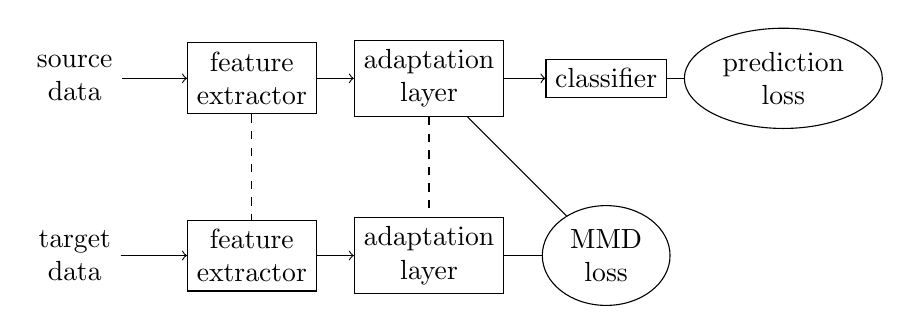
\begin{tikzpicture}[node distance=2.25cm]
				\node (src) [data] {source\\data};
				\node (trg) [data, below of=src] {target\\data};
				\node (fe1) [block,right of=src] {feature\\extractor};
				\node (fe2) [block,right of=trg] {feature\\extractor};
				\node (al1) [block,right of=fe1] {adaptation\\layer};
				\node (al2) [block,right of=fe2] {adaptation\\layer};
				\node (clf) [block,right of=al1] {classifier};
				\node (loss) [loss,right of=clf] {prediction\\loss};
				\node (mmd) [loss,right of=al2] {MMD\\loss};
				\draw [->] (src) -- (fe1);
				\draw [->] (trg) -- (fe2);
				\draw [->] (fe1) -- (al1);
				\draw [->] (fe2) -- (al2);
				\draw [->] (al1) -- (clf);
				\draw [dashed] (fe1) -- (fe2);
				\draw [dashed] (al1) -- (al2);
				\draw (clf) -- (loss);
				\draw (al1) -- (mmd);
				\draw (al2) -- (mmd);
			\end{tikzpicture}
		\end{center}
	\end{figure}
}
\frame{
	\frametitle{Deep Correlation Alignment\footfullcite{sun2016} (Deep CORAL)}
	\begin{figure}
		\begin{center}
			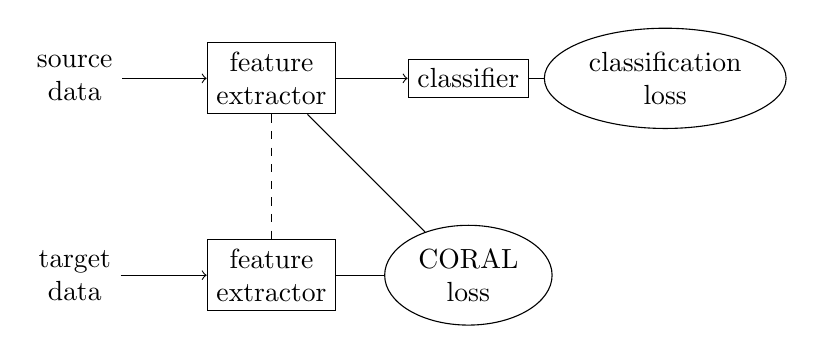
\begin{tikzpicture}[node distance=2.5cm]
				\node (src) [data] {source\\data};
				\node (trg) [data, below of=src] {target\\data};
				\node (fe1) [block,right of=src] {feature\\extractor};
				\node (fe2) [block,right of=trg] {feature\\extractor};
				\node (clf) [block,right of=fe1] {classifier};
				\node (loss) [loss,right of=clf] {classification\\loss};
				\node (coral) [loss,right of=fe2] {CORAL\\loss};
				\draw [->] (src) -- (fe1);
				\draw [->] (trg) -- (fe2);
				\draw [->] (fe1) -- (clf);
				\draw [dashed] (fe1) -- (fe2);
				\draw (clf) -- (loss);
				\draw (fe1) -- (coral);
				\draw (fe2) -- (coral);
			\end{tikzpicture}
		\end{center}
	\end{figure}
}
\frame{
	\frametitle{Domain-Adversarial Neural Network\footfullcite{ganin2016} (DANN)}
	\begin{figure}
		\begin{center}
			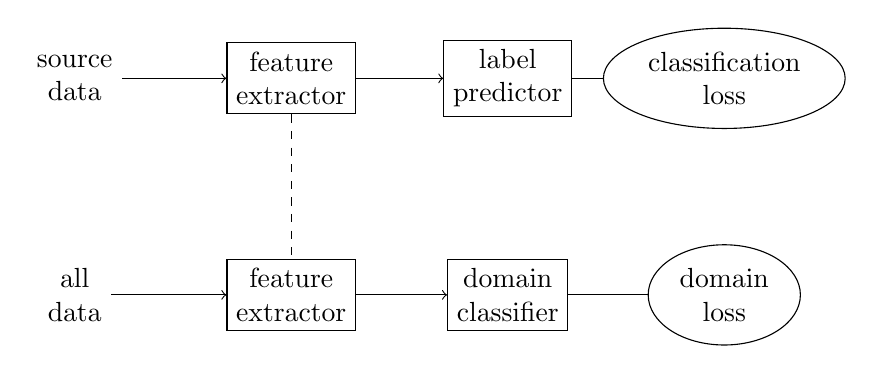
\begin{tikzpicture}[node distance=2.75cm]
				\node (src) [data] {source\\data};
				\node (all) [data, below of=src] {all\\data};
				\node (fe1) [block,right of=src] {feature\\extractor};
				\node (fe2) [block,right of=all] {feature\\extractor};
				\node (clf) [block,right of=fe1] {label\\predictor};
				\node (dom) [block,right of=fe2] {domain\\classifier};
				\node (clf_loss) [loss,right of=clf] {classification\\loss};
				\node (dom_loss) [loss,right of=dom] {domain\\loss};
				\draw [->] (src) -- (fe1);
				\draw [->] (all) -- (fe2);
				\draw [->] (fe1) -- (clf);
				\draw [->] (fe2) -- (dom);
				\draw [dashed] (fe1) -- (fe2);
				\draw (clf) -- (clf_loss);
				\draw (dom) -- (dom_loss);
			\end{tikzpicture}
		\end{center}
	\end{figure}
}
\frame{
	\frametitle{Deep Reconstruction-Classification Network\footfullcite{ghifary2016} (DRCN)}
	\begin{figure}
		\begin{center}
			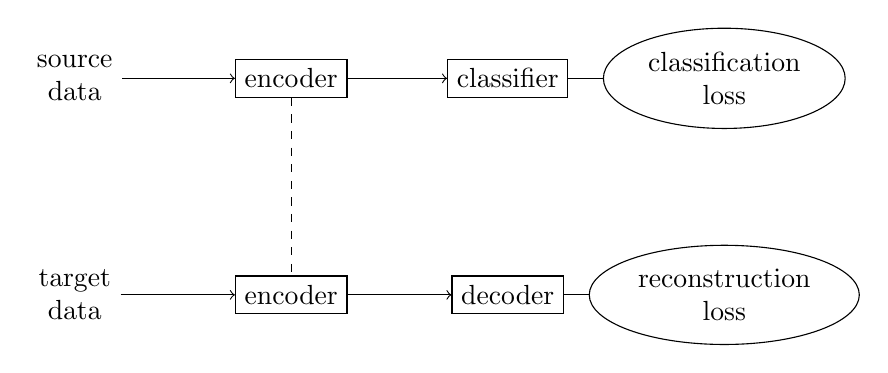
\begin{tikzpicture}[node distance=2.75cm]
				\node (src) [data] {source\\data};
				\node (trg) [data, below of=src] {target\\data};
				\node (enc1) [block,right of=src] {encoder};
				\node (enc2) [block,right of=trg] {encoder};
				\node (clf) [block,right of=enc1] {classifier};
				\node (dec) [block,right of=enc2] {decoder};
				\node (clf_loss) [loss,right of=clf] {classification\\loss};
				\node (rec_loss) [loss,right of=dec] {reconstruction\\loss};
				\draw [->] (src) -- (enc1);
				\draw [->] (trg) -- (enc2);
				\draw [->] (enc1) -- (clf);
				\draw [->] (enc2) -- (dec);
				\draw [dashed] (enc1) -- (enc2);
				\draw (clf) -- (clf_loss);
				\draw (dec) -- (rec_loss);
			\end{tikzpicture}
		\end{center}
	\end{figure}
}
\section{Experiments in SDSS and LAMOST Survey}
\frame{
	\frametitle{Experimental Results}
	\begin{figure}
		\begin{center}
			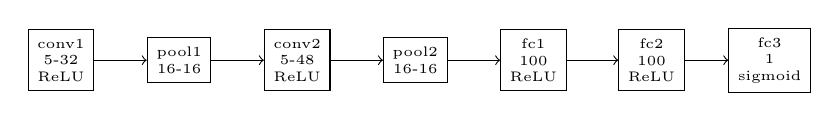
\begin{tikzpicture}[node distance=1.5cm]
				\node (conv1) [layer] {conv1\\5-32\\ReLU};
				\node (pool1) [layer,right of=conv1] {pool1\\16-16};
				\node (conv2) [layer,right of=pool1] {conv2\\5-48\\ReLU};
				\node (pool2) [layer,right of=conv2] {pool2\\16-16};
				\node (fc1) [layer,right of=pool2] {fc1\\100\\ReLU};
				\node (fc2) [layer,right of=fc1] {fc2\\100\\ReLU};
				\node (fc3) [layer,right of=fc2] {fc3\\1\\sigmoid};
				\draw [->] (conv1) -- (pool1);
				\draw [->] (pool1) -- (conv2);
				\draw [->] (conv2) -- (pool2);
				\draw [->] (pool2) -- (fc1);
				\draw [->] (fc1) -- (fc2);
				\draw [->] (fc2) -- (fc3);
			\end{tikzpicture}
		\end{center}
		\caption{The baseline model is an adapted LeNet-5.}
	\end{figure}
	\begin{table}
		\begin{tabular}{|l|r|r|r|r|}
			\hline
			Method & Source \(F_1\) & Target \(F_1\) & Precision (\%) & Recall (\%) \\
			\hline \hline
			baseline & 0.9397 & 0.2294 & 13.48 & 76.84 \\ \hline
			DDC & 0.9354 & 0.2005 & 11.51 & 77.89 \\ \hline
			Deep CORAL & 0.9396 & 0.2509 & 14.97 & 77.37 \\ \hline
			DANN & \multicolumn{4}{c|}{did not converge} \\ \hline
			DRCN & 0.9393 & 0.2898 & 17.97 & 74.74 \\ \hline
		\end{tabular}
		\caption{Summary table of results of experiments}
	\end{table}
}
\section{Problems of Scientific Data}
\frame{
	\frametitle{Problems of Scientific Data}
	The methods did not achieve satisfoctory results although:
	\begin{enumerate}
		\item Dimensionality reduction shows discrepancy of distributions.
		\item Statistics of the methods (MMD and CORAL are low, reconstruction works properly).
	\end{enumerate}
	\begin{alertblock}{The cause of failure}
		Imperfect and noisy datasets that is proved by \textit{misclassifications}.
	\end{alertblock}
}
\frame{
	\frametitle{Misclassifications in the Datasets}
	\begin{figure}
		\subfloat[Source false positive but is clearly QSO.]{
			\includegraphics[width=\textwidth]{img/src_fp/spec-0560-52296-0199.pdf}
		}\\
		\subfloat[Target false positive but contains bad pixels.]{
			\includegraphics[width=\textwidth]{img/trg_fp/spec-56225-GAC051N24B1_sp10-104.pdf}
		}
	\end{figure}
}
\frame{
	\frametitle{Suggested Solutions}
	\begin{enumerate}
		\item New more robust architectures or learning algorithms.
		\item Automatic preprocessing algorithms based on machine learning.
	\end{enumerate}
}
\end{document}
